\documentclass{standalone}
\usepackage{tikz}
\usetikzlibrary{patterns, positioning}


\begin{document}
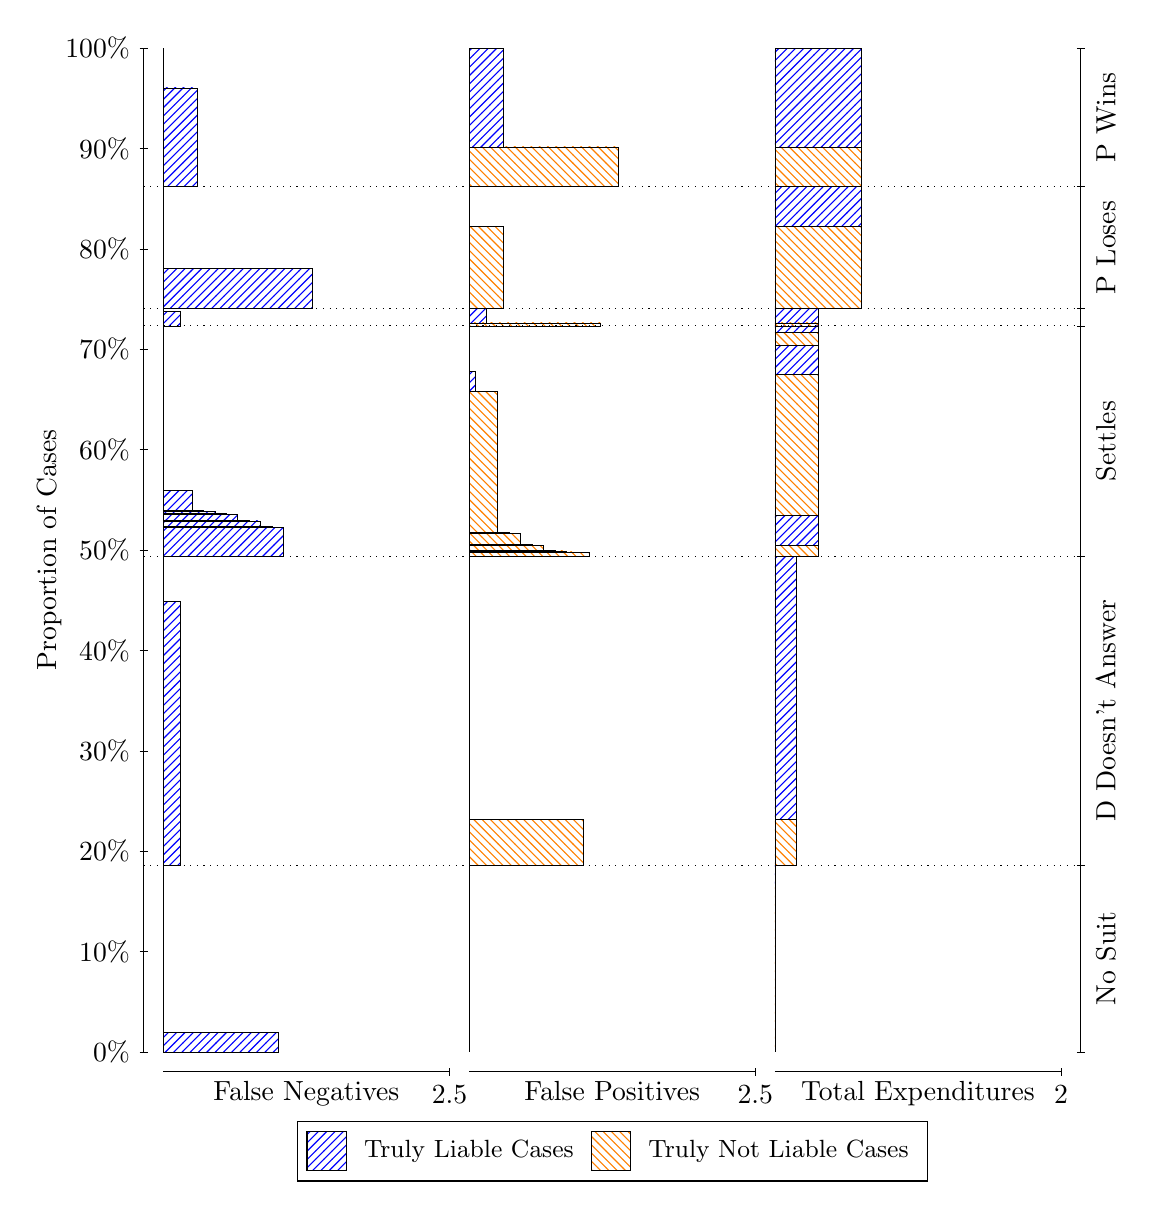
\begin{tikzpicture}
\draw[black, very thin] (1.5,1.75) -- (1.5,14.5);
\node[rotate=90, text=black, anchor=center] at (0.3, 8.125) {Proportion of Cases};
\draw[black, very thin] (1.45,1.75) -- (1.55,1.75);
\node[text=black, anchor=east] at (1.45, 1.75) {0\%};
\draw[black, very thin] (1.45,3.025) -- (1.55,3.025);
\node[text=black, anchor=east] at (1.45, 3.025) {10\%};
\draw[black, very thin] (1.45,4.3) -- (1.55,4.3);
\node[text=black, anchor=east] at (1.45, 4.3) {20\%};
\draw[black, very thin] (1.45,5.575) -- (1.55,5.575);
\node[text=black, anchor=east] at (1.45, 5.575) {30\%};
\draw[black, very thin] (1.45,6.85) -- (1.55,6.85);
\node[text=black, anchor=east] at (1.45, 6.85) {40\%};
\draw[black, very thin] (1.45,8.125) -- (1.55,8.125);
\node[text=black, anchor=east] at (1.45, 8.125) {50\%};
\draw[black, very thin] (1.45,9.4) -- (1.55,9.4);
\node[text=black, anchor=east] at (1.45, 9.4) {60\%};
\draw[black, very thin] (1.45,10.675) -- (1.55,10.675);
\node[text=black, anchor=east] at (1.45, 10.675) {70\%};
\draw[black, very thin] (1.45,11.95) -- (1.55,11.95);
\node[text=black, anchor=east] at (1.45, 11.95) {80\%};
\draw[black, very thin] (1.45,13.225) -- (1.55,13.225);
\node[text=black, anchor=east] at (1.45, 13.225) {90\%};
\draw[black, very thin] (1.45,14.5) -- (1.55,14.5);
\node[text=black, anchor=east] at (1.45, 14.5) {100\%};

\draw[black, very thin] (13.4,1.75) -- (13.4,14.5);
\draw[black, very thin] (13.35,1.75) -- (13.45,1.75);
\node[anchor=west] at (13.35, 1.75) {};
\draw[black, very thin] (13.35,4.1224) -- (13.45,4.1224);
\node[anchor=west] at (13.35, 4.1224) {};
\draw[black, very thin] (13.35,8.0462) -- (13.45,8.0462);
\node[anchor=west] at (13.35, 8.0462) {};
\draw[black, very thin] (13.35,10.972) -- (13.45,10.972);
\node[anchor=west] at (13.35, 10.972) {};
\draw[black, very thin] (13.35,11.192) -- (13.45,11.192);
\node[anchor=west] at (13.35, 11.192) {};
\draw[black, very thin] (13.35,12.738) -- (13.45,12.738);
\node[anchor=west] at (13.35, 12.738) {};
\draw[black, very thin] (13.35,14.5) -- (13.45,14.5);
\node[anchor=west] at (13.35, 14.5) {};

\draw[black, very thin, pattern color=blue, pattern=north east lines] (1.75,1.75) rectangle (3.2033,1.9996);
\draw[black, very thin, pattern color=orange, pattern=north west lines] (1.75,1.9996) rectangle (1.75,4.1224);
\draw[black, very thin, pattern color=blue, pattern=north east lines] (1.75,4.1224) rectangle (1.968,7.4689);
\draw[black, very thin, pattern color=orange, pattern=north west lines] (1.75,7.4689) rectangle (1.75,8.0462);
\draw[black, very thin, pattern color=blue, pattern=north east lines] (1.75,8.0462) rectangle (3.276,8.4161);
\draw[black, very thin, pattern color=blue, pattern=north east lines] (1.75,8.4161) rectangle (3.1307,8.4245);
\draw[black, very thin, pattern color=blue, pattern=north east lines] (1.75,8.4245) rectangle (2.9853,8.4947);
\draw[black, very thin, pattern color=blue, pattern=north east lines] (1.75,8.4947) rectangle (2.84,8.5037);
\draw[black, very thin, pattern color=blue, pattern=north east lines] (1.75,8.5037) rectangle (2.6947,8.5771);
\draw[black, very thin, pattern color=blue, pattern=north east lines] (1.75,8.5771) rectangle (2.5493,8.5871);
\draw[black, very thin, pattern color=blue, pattern=north east lines] (1.75,8.5871) rectangle (2.404,8.6147);
\draw[black, very thin, pattern color=blue, pattern=north east lines] (1.75,8.6147) rectangle (2.2587,8.6254);
\draw[black, very thin, pattern color=blue, pattern=north east lines] (1.75,8.6254) rectangle (2.1133,8.8821);
\draw[black, very thin, pattern color=orange, pattern=north west lines] (1.75,8.8821) rectangle (1.75,10.972);
\draw[black, very thin, pattern color=blue, pattern=north east lines] (1.75,10.972) rectangle (1.968,11.154);
\draw[black, very thin, pattern color=orange, pattern=north west lines] (1.75,11.154) rectangle (1.75,11.192);
\draw[black, very thin, pattern color=blue, pattern=north east lines] (1.75,11.192) rectangle (3.6393,11.697);
\draw[black, very thin, pattern color=orange, pattern=north west lines] (1.75,11.697) rectangle (1.75,12.738);
\draw[black, very thin, pattern color=blue, pattern=north east lines] (1.75,12.738) rectangle (2.186,13.994);
\draw[black, very thin, pattern color=orange, pattern=north west lines] (1.75,13.994) rectangle (1.75,14.5);
\draw[black, very thin, pattern color=orange, pattern=north west lines] (5.6333,1.75) rectangle (5.6333,3.8728);
\draw[black, very thin, pattern color=blue, pattern=north east lines] (5.6333,3.8728) rectangle (5.6333,4.1224);
\draw[black, very thin, pattern color=orange, pattern=north west lines] (5.6333,4.1224) rectangle (7.0867,4.6998);
\draw[black, very thin, pattern color=blue, pattern=north east lines] (5.6333,4.6998) rectangle (5.6333,8.0462);
\draw[black, very thin, pattern color=orange, pattern=north west lines] (5.6333,8.0462) rectangle (7.1593,8.0951);
\draw[black, very thin, pattern color=orange, pattern=north west lines] (5.6333,8.0951) rectangle (7.014,8.1);
\draw[black, very thin, pattern color=orange, pattern=north west lines] (5.6333,8.1) rectangle (6.8687,8.1125);
\draw[black, very thin, pattern color=orange, pattern=north west lines] (5.6333,8.1125) rectangle (6.7233,8.117);
\draw[black, very thin, pattern color=orange, pattern=north west lines] (5.6333,8.117) rectangle (6.578,8.1851);
\draw[black, very thin, pattern color=orange, pattern=north west lines] (5.6333,8.1851) rectangle (6.4327,8.1941);
\draw[black, very thin, pattern color=orange, pattern=north west lines] (5.6333,8.1941) rectangle (6.2873,8.3386);
\draw[black, very thin, pattern color=orange, pattern=north west lines] (5.6333,8.3386) rectangle (6.142,8.347);
\draw[black, very thin, pattern color=orange, pattern=north west lines] (5.6333,8.347) rectangle (5.9967,10.136);
\draw[black, very thin, pattern color=blue, pattern=north east lines] (5.6333,10.136) rectangle (5.706,10.393);
\draw[black, very thin, pattern color=blue, pattern=north east lines] (5.6333,10.393) rectangle (5.6333,10.972);
\draw[black, very thin, pattern color=orange, pattern=north west lines] (5.6333,10.972) rectangle (7.3047,11.01);
\draw[black, very thin, pattern color=blue, pattern=north east lines] (5.6333,11.01) rectangle (5.8513,11.192);
\draw[black, very thin, pattern color=orange, pattern=north west lines] (5.6333,11.192) rectangle (6.0693,12.233);
\draw[black, very thin, pattern color=blue, pattern=north east lines] (5.6333,12.233) rectangle (5.6333,12.738);
\draw[black, very thin, pattern color=orange, pattern=north west lines] (5.6333,12.738) rectangle (7.5227,13.244);
\draw[black, very thin, pattern color=blue, pattern=north east lines] (5.6333,13.244) rectangle (6.0693,14.5);
\draw[black, very thin, pattern color=orange, pattern=north west lines] (9.5167,1.75) rectangle (9.5167,3.8728);
\draw[black, very thin, pattern color=blue, pattern=north east lines] (9.5167,3.8728) rectangle (9.5167,4.1224);
\draw[black, very thin, pattern color=orange, pattern=north west lines] (9.5167,4.1224) rectangle (9.7892,4.6998);
\draw[black, very thin, pattern color=blue, pattern=north east lines] (9.5167,4.6998) rectangle (9.7892,8.0462);
\draw[black, very thin, pattern color=orange, pattern=north west lines] (9.5167,8.0462) rectangle (10.062,8.1851);
\draw[black, very thin, pattern color=blue, pattern=north east lines] (9.5167,8.1851) rectangle (10.062,8.5636);
\draw[black, very thin, pattern color=orange, pattern=north west lines] (9.5167,8.5636) rectangle (10.062,10.353);
\draw[black, very thin, pattern color=blue, pattern=north east lines] (9.5167,10.353) rectangle (10.062,10.722);
\draw[black, very thin, pattern color=orange, pattern=north west lines] (9.5167,10.722) rectangle (10.062,10.884);
\draw[black, very thin, pattern color=blue, pattern=north east lines] (9.5167,10.884) rectangle (10.062,10.972);
\draw[black, very thin, pattern color=orange, pattern=north west lines] (9.5167,10.972) rectangle (10.062,11.01);
\draw[black, very thin, pattern color=blue, pattern=north east lines] (9.5167,11.01) rectangle (10.062,11.192);
\draw[black, very thin, pattern color=orange, pattern=north west lines] (9.5167,11.192) rectangle (10.607,12.233);
\draw[black, very thin, pattern color=blue, pattern=north east lines] (9.5167,12.233) rectangle (10.607,12.738);
\draw[black, very thin, pattern color=orange, pattern=north west lines] (9.5167,12.738) rectangle (10.607,13.244);
\draw[black, very thin, pattern color=blue, pattern=north east lines] (9.5167,13.244) rectangle (10.607,14.5);
\draw[black, dotted] (1.5,4.1224) -- (13.4,4.1224);
\draw[black, dotted] (1.5,8.0462) -- (13.4,8.0462);
\draw[black, dotted] (1.5,10.972) -- (13.4,10.972);
\draw[black, dotted] (1.5,11.192) -- (13.4,11.192);
\draw[black, dotted] (1.5,12.738) -- (13.4,12.738);
\draw[black, very thin] (1.75,1.5) -- (5.3833,1.5);
\node[text=black, anchor=north] at (3.5667, 1.5) {False Negatives};
\draw[black, very thin] (5.3833,1.45) -- (5.3833,1.55);
\node[text=black, anchor=north] at (5.3833, 1.45) {2.5};

\draw[black, very thin] (5.6333,1.5) -- (9.2667,1.5);
\node[text=black, anchor=north] at (7.45, 1.5) {False Positives};
\draw[black, very thin] (9.2667,1.45) -- (9.2667,1.55);
\node[text=black, anchor=north] at (9.2667, 1.45) {2.5};

\draw[black, very thin] (9.5167,1.5) -- (13.15,1.5);
\node[text=black, anchor=north] at (11.333, 1.5) {Total Expenditures};
\draw[black, very thin] (13.15,1.45) -- (13.15,1.55);
\node[text=black, anchor=north] at (13.15, 1.45) {2};

\node[text=black, centered, rotate=90] at (13.72, 2.9362) {No Suit};
\node[text=black, centered, rotate=90] at (13.72, 6.0843) {D Doesn't Answer};
\node[text=black, centered, rotate=90] at (13.72, 9.509) {Settles};

\node[text=black, centered, rotate=90] at (13.72, 11.965) {P Loses};
\node[text=black, centered, rotate=90] at (13.72, 13.619) {P Wins};

\draw (7.449999999999999,1.5) node[draw=none] (baseCoordinate) {};
\begin{scope}[align=center]
        \matrix[scale=0.5, draw=black, below=0.5cm of baseCoordinate, nodes={draw}, column sep=0.1cm]{
            \node[rectangle, draw, minimum width=0.5cm, minimum height=0.5cm, pattern color=blue, pattern=north east lines] {}; &
            \node[draw=none, font=\small, text=black] (B) {Truly Liable Cases}; &
            \node[rectangle, draw, minimum width=0.5cm, minimum height=0.5cm, pattern color=orange, pattern=north west lines] {}; &
            \node[draw=none, font=\small, text=black] (B) {Truly Not Liable Cases}; \\
            };
\end{scope}

\end{tikzpicture}
\end{document}